%-----------------------------------
% TITLE PAGE
%-----------------------------------

\title[大数据分析与数学建模]{\texorpdfstring{\LARGE \bfseries 大数据分析与数学建模}{大数据分析与数学建模}}
\author[线性模型基础(2)]
{\Large \bfseries 第一章\quad 线性代数与线性模型基础 \\ \vspace{0.5em} \large \S 1.3 线性模型的一般形式 \quad \S 1.4 回归与方差分析的矩阵表示}
\date{}

%------------------------------------------------

\begin{document}

%------------------------------------------------

\begin{frame}
\titlepage
\end{frame}

%------------------------------------------------

\begin{frame}
\frametitle{内容提要}
\tableofcontents
\end{frame}

%-----------------------------------
% PRESENTATION SLIDES
%-----------------------------------

\section[复习]{复习：线性代数基础}

%------------------------------------------------

\begin{frame}
\frametitle{复习：矩阵运算核心}

在进入线性模型之前，我们快速回顾一下上节课的核心工具：

\begin{enumerate}
    \item \textbf{矩阵乘法}：$C = AB$，其中 $C_{ij} = (\text{Row } i \text{ of } A) \cdot (\text{Col } j \text{ of } B)$。
    \begin{itemize}
        \item 结合律成立 $(AB)C = A(BC)$，
        \item 但\textbf{交换律一般不成立} $AB \neq BA$。
    \end{itemize}
    \item \textbf{转置 (Transpose)}：行列互换。
    \begin{itemize}
        \item 关键性质：$(AB)^T = B^T A^T$ （穿脱衣法则）。
        \item 对称阵：$A^T = A$。$X^T X$ 永远是对称阵。
    \end{itemize}
    \item \textbf{逆矩阵 (Inverse)}：$A A^{-1} = I$。
    \begin{itemize}
        \item 只有方阵且满秩时才可逆。
        \item $(AB)^{-1} = B^{-1} A^{-1}$。
    \end{itemize}
\end{enumerate}

\end{frame}

%------------------------------------------------

\begin{frame}
\frametitle{复习：列空间与秩}

\begin{block}{列空间 (Column Space) $\mathcal{C}(A)$}
矩阵 $A$ 的所有列向量的线性组合构成的空间。
\[
A\mathbf{x} = x_1 \mathbf{a}_1 + x_2 \mathbf{a}_2 + \dots + x_n \mathbf{a}_n
\]
方程 $A\mathbf{x} = \mathbf{b}$ 有解当且仅当 $\mathbf{b} \in \mathcal{C}(A)$。
\end{block}

\begin{block}{秩 (Rank)}
矩阵中线性无关的列（或行）的最大数目。
\begin{itemize}
    \item 若 $A$ 是 $n \times p$ 矩阵 ($n > p$)，且 $\text{rank}(A) = p$，称 $A$ \textbf{列满秩}。
    \item 只有列满秩时，$A^T A$ 才可逆，这是最小二乘法有唯一解的前提。
\end{itemize}
\end{block}

\end{frame}

%------------------------------------------------

\section[线性模型]{线性模型的一般形式}

%------------------------------------------------

\begin{frame}
\frametitle{什么是线性模型？}

在统计学与数据科学中，\textbf{线性模型} (Linear Model) 是应用最广泛的建模工具。
它描述了响应变量 $\mathbf{y}$ 与一组解释变量（特征）之间的线性关系。

\[
\mathbf{y} = X \boldsymbol{\beta} + \boldsymbol{\epsilon}
\]

\begin{itemize}
    \item $\mathbf{y}$: $n \times 1$ 观测向量 (Response / Dependent Variable)。
    \item $X$: $n \times p$ \textbf{设计矩阵} (Design Matrix)。
    \item $\boldsymbol{\beta}$: $p \times 1$ 未知参数向量 (Parameters / Effects)。
    \item $\boldsymbol{\epsilon}$: $n \times 1$ 随机误差向量 (Error / Residuals)，通常假设 $\boldsymbol{\epsilon} \sim N(\mathbf{0}, \sigma^2 I)$。
\end{itemize}

\end{frame}

%------------------------------------------------

\begin{frame}
\frametitle{设计矩阵 (Design Matrix) 的核心地位}

模型的核心在于如何构造设计矩阵 $X$。

\[
X = \begin{pmatrix}
1 & x_{11} & x_{12} & \cdots & x_{1k} \\
1 & x_{21} & x_{22} & \cdots & x_{2k} \\
\vdots & \vdots & \vdots & \ddots & \vdots \\
1 & x_{n1} & x_{n2} & \cdots & x_{nk}
\end{pmatrix}
\]

\begin{itemize}
    \item 第一列通常全是 1，对应的参数 $\beta_0$ 是\textbf{截距} (Intercept) 或总均值。
    \item 后续列可以是连续变量（如体重、日龄），也可以是分类变量的编码（如品种、性别）。
    \item \textbf{建模的本质，就是构造 $X$ 矩阵。}
\end{itemize}

\end{frame}

%------------------------------------------------

\begin{frame}
\frametitle{最小二乘估计 (Ordinary Least Squares, OLS)}

我们的目标是找到 $\boldsymbol{\beta}$ 的估计值 $\hat{\boldsymbol{\beta}}$，使得模型预测值 $\hat{\mathbf{y}} = X \hat{\boldsymbol{\beta}}$ 与真实值 $\mathbf{y}$ 之间的误差平方和最小：

\[
Q(\boldsymbol{\beta}) = \|\mathbf{y} - X \boldsymbol{\beta}\|^2 = (\mathbf{y} - X \boldsymbol{\beta})^T (\mathbf{y} - X \boldsymbol{\beta}) \to \min
\]

\pause

\begin{block}{正规方程 (Normal Equations)}
通过几何投影（\S\,3）或代数求导（\S\,4）均可推导出：
\[
X^T X \hat{\boldsymbol{\beta}} = X^T \mathbf{y}
\]
\end{block}

\begin{block}{OLS 解}
若 $X$ 列满秩（Rank = $p$），则 $X^T X$ 可逆，唯一解为：
\[
\hat{\boldsymbol{\beta}} = (X^T X)^{-1} X^T \mathbf{y}
\]
\end{block}

\end{frame}

%------------------------------------------------

\section[几何视角]{从几何视角看最小二乘法}

%------------------------------------------------

\begin{frame}
\frametitle{矛盾的方程组}

在实际数据分析中，我们往往面临\textbf{超定方程组} (Overdetermined System)：
\[
X \boldsymbol{\beta} = \mathbf{y}
\]
其中 $n \gg p$（样本量远大于参数个数）。

\begin{itemize}
    \item 观测向量 $\mathbf{y}$ 通常不在 $X$ 的列空间 $\mathcal{C}(X)$ 中（因为存在随机误差 $\boldsymbol{\epsilon}$）。
    \item 这意味着方程 $X \boldsymbol{\beta} = \mathbf{y}$ \textbf{无解}。
\end{itemize}

\vspace{1em}
\textbf{核心思想}：
既然找不到完美的 $\boldsymbol{\beta}$ 使得 $X \boldsymbol{\beta}$ 等于 $\mathbf{y}$，那我们就退而求其次：
找一个 $\hat{\boldsymbol{\beta}}$，使得 $X \hat{\boldsymbol{\beta}}$ \textbf{最接近} $\mathbf{y}$。

\end{frame}

%------------------------------------------------

\begin{frame}
\frametitle{几何解释：投影 (Projection)}

最小二乘法的几何本质是\textbf{正交投影}。

\begin{itemize}
    \item 我们寻找 $\mathcal{C}(X)$ 中距离 $\mathbf{y}$ 最近的点 $\hat{\mathbf{y}}$。
    \item 最短距离对应于\textbf{垂线}。即残差向量 $\mathbf{e} = \mathbf{y} - \hat{\mathbf{y}}$ 必须垂直于 $\mathcal{C}(X)$。
\end{itemize}

\begin{center}
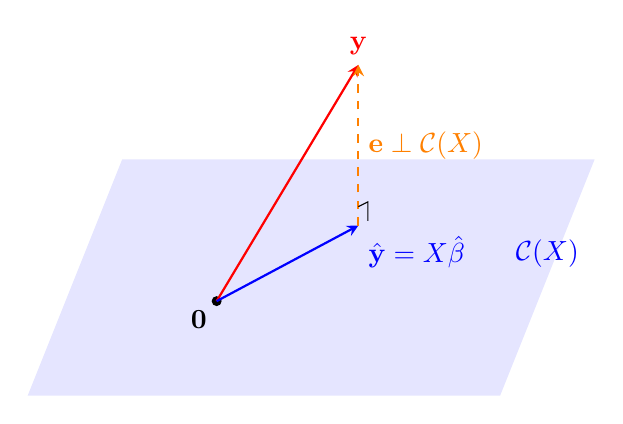
\begin{tikzpicture}[scale=1.2, >=stealth]
    % Draw plane representing column space of X
    \fill[blue!10] (-2, -1) -- (3, -1) -- (4, 1.5) -- (-1, 1.5) -- cycle;
    \node[blue] at (3.5, 0.5) {$\mathcal{C}(X)$};

    % Origin
    \coordinate (O) at (0,0);
    \fill (O) circle (1.5pt) node[below left] {$\mathbf{0}$};

    % Vectors
    \draw[->, thick, red] (O) -- (1.5, 2.5) node[above] {$\mathbf{y}$};
    \draw[->, thick, blue] (O) -- (1.5, 0.8) node[below right] {$\hat{\mathbf{y}} = X\hat{\boldsymbol{\beta}}$};
    \draw[->, thick, dashed, orange] (1.5, 0.8) -- (1.5, 2.5) node[midway, right] {$\mathbf{e} \perp \mathcal{C}(X)$};

    % Right angle symbol
    \draw (1.5, 1.0) -- (1.6, 1.05) -- (1.6, 0.85);
\end{tikzpicture}
\end{center}

\end{frame}

%------------------------------------------------

\begin{frame}
\frametitle{从几何直觉导出正规方程}

利用几何条件：\textbf{残差 $\mathbf{e}$ 垂直于 $X$ 的每一列}。
即 $\mathbf{e}$ 垂直于 $\mathcal{C}(X)$ 中的任意向量。

\[
X^T \mathbf{e} = \mathbf{0}
\]

代入 $\mathbf{e} = \mathbf{y} - X \hat{\boldsymbol{\beta}}$：

\[
X^T (\mathbf{y} - X \hat{\boldsymbol{\beta}}) = \mathbf{0}
\]

展开整理：
\[
X^T \mathbf{y} - X^T X \hat{\boldsymbol{\beta}} = \mathbf{0} \implies X^T X \hat{\boldsymbol{\beta}} = X^T \mathbf{y}
\]

\begin{alertblock}{结论}
这再次得到了\textbf{正规方程}！
无需复杂的微积分求导，仅凭几何直觉 ($\mathbf{e} \perp \mathcal{C}(X)$) 就能得到相同的结果。
\end{alertblock}

\end{frame}

%------------------------------------------------

\section[代数推导]{最小二乘法的代数推导}

%------------------------------------------------

\begin{frame}
\frametitle{最小二乘目标函数展开}

最小化误差平方和：

\[
Q(\boldsymbol{\beta}) = (\mathbf{y} - X\boldsymbol{\beta})^T (\mathbf{y} - X\boldsymbol{\beta})
\]

展开利用矩阵转置性质 $(AB)^T = B^T A^T$：
\[
\begin{aligned}
Q(\boldsymbol{\beta}) &= (\mathbf{y}^T - \boldsymbol{\beta}^T X^T) (\mathbf{y} - X\boldsymbol{\beta}) \\
&= \mathbf{y}^T\mathbf{y} - \mathbf{y}^T X\boldsymbol{\beta} - \boldsymbol{\beta}^T X^T \mathbf{y} + \boldsymbol{\beta}^T X^T X \boldsymbol{\beta}
\end{aligned}
\]

注意 $\mathbf{y}^T X\boldsymbol{\beta}$ 是一个标量，其转置等于自身：
\[
(\mathbf{y}^T X\boldsymbol{\beta})^T = \boldsymbol{\beta}^T X^T \mathbf{y}
\]
所以：
\[
Q(\boldsymbol{\beta}) = \mathbf{y}^T\mathbf{y} - 2\boldsymbol{\beta}^T X^T \mathbf{y} + \boldsymbol{\beta}^T X^T X \boldsymbol{\beta}
\]

这是一个关于 $\boldsymbol{\beta}$ 的二次函数。
\end{frame}

%------------------------------------------------

\begin{frame}
\frametitle{求导得到正规方程}

我们需要利用矩阵微分公式：
\begin{enumerate}
    \item $\frac{\partial (\mathbf{a}^T \mathbf{x})}{\partial \mathbf{x}} = \mathbf{a}$
    \item $\frac{\partial (\mathbf{x}^T A \mathbf{x})}{\partial \mathbf{x}} = (A + A^T)\mathbf{x}$，若 $A$ 对称，则为 $2A\mathbf{x}$。
\end{enumerate}

\vspace{1em}
对 $Q(\boldsymbol{\beta})$ 关于 $\boldsymbol{\beta}$ 求导：
\[
\frac{\partial Q}{\partial \boldsymbol{\beta}} = -2X^T \mathbf{y} + 2(X^T X)\boldsymbol{\beta}
\]

令导数为 $\mathbf{0}$：
\[
-2X^T \mathbf{y} + 2X^T X \hat{\boldsymbol{\beta}} = \mathbf{0} \implies X^T X \hat{\boldsymbol{\beta}} = X^T \mathbf{y}
\]

这称为\textbf{正规方程 (Normal Equations)}。
\end{frame}

%------------------------------------------------

\section[统计推断]{OLS 的统计性质与模型评估}

%------------------------------------------------

\begin{frame}
\frametitle{本节导图：拿到 $\hat{\boldsymbol{\beta}}$ 之后}

我们已经得到 OLS 估计量 $\hat{\boldsymbol{\beta}} = (X^TX)^{-1}X^T\mathbf{y}$，接下来自然要问三个问题：

\begin{enumerate}
    \item \textbf{几何上}：预测值 $\hat{\mathbf{y}}$ 和残差 $\mathbf{e}$ 的本质是什么？
    \begin{itemize}\item 引出\textbf{投影矩阵} $H$，以及残差的正交性。\end{itemize}
    \item \textbf{统计上}：$\hat{\boldsymbol{\beta}}$ 有多可靠？$\sigma^2$ 如何从数据中估计？
    \begin{itemize}\item 引出 \textbf{Gauss-Markov 定理}与参数方差公式。\end{itemize}
    \item \textbf{评估上}：模型拟合得好不好？某个变量是否真的显著？
    \begin{itemize}\item 引出 \textbf{方差分解}、$R^2$ 与 $t$ 检验。\end{itemize}
\end{enumerate}

\end{frame}

%------------------------------------------------

\begin{frame}
\frametitle{投影矩阵 (Projection Matrix)}

我们的预测值是 $\hat{\mathbf{y}} = X \hat{\boldsymbol{\beta}}$。将 $\hat{\boldsymbol{\beta}} = (X^T X)^{-1} X^T \mathbf{y}$ 代入：

\[
\hat{\mathbf{y}} = X (X^T X)^{-1} X^T \mathbf{y} = H \mathbf{y}
\]

其中定义 $H$ 为\textbf{投影矩阵} (Projection Matrix)，统计学中常称为\textbf{帽子矩阵} (Hat Matrix)：
\[
H = X (X^T X)^{-1} X^T
\]
因为它将观测值 $\mathbf{y}$ 正交投影到了 $X$ 的列空间中，得到预测值 $\hat{\mathbf{y}}$。

\end{frame}

%------------------------------------------------

\begin{frame}
\frametitle{投影矩阵 $H$ 的性质}

$H$ 具有优良的数学性质：

\begin{enumerate}
    \item \textbf{对称性}：
    \[
    H^T = (X (X^T X)^{-1} X^T)^T = X \underbrace{((X^T X)^{-1})^T}_{= (X^TX)^{-1}} X^T = H
    \]
    （因为 $X^TX$ 是对称阵，其逆仍对称：$((X^TX)^{-1})^T = ((X^TX)^T)^{-1} = (X^TX)^{-1}$。）

    \item \textbf{幂等性}：
    \[
    H^2 = H H = X (X^T X)^{-1} \underbrace{X^T X (X^T X)^{-1}}_{= I} X^T = X(X^TX)^{-1}X^T = H
    \]
\end{enumerate}

\begin{itemize}
    \item $H$ 是将任意向量投影到 $X$ 的列空间 $\mathcal{C}(X)$ 上的\textbf{正交投影矩阵}。
    \item \textbf{重要性质}：
    \[ \text{rank}(H) = \text{tr}(H) = p \]
    这意味着 $H$ 的迹等于模型参数的个数（自由度），这是统计推断的核心桥梁。
\end{itemize}
\end{frame}

%------------------------------------------------

\begin{frame}
\frametitle{残差向量与正交性}

\textbf{残差} (Residuals) 定义为观测值与预测值之差：
\[
\mathbf{e} = \mathbf{y} - \hat{\mathbf{y}} = \mathbf{y} - H\mathbf{y} = (I - H)\mathbf{y}
\]

\textbf{性质}：残差与设计矩阵的列空间正交，即与\textbf{所有解释变量正交}。

注意到 $X^T H = X^T X (X^T X)^{-1} X^T = I \cdot X^T = X^T$，因此：
\[
X^T \mathbf{e} = X^T (I - H)\mathbf{y} = (X^T - X^T H)\mathbf{y} = (X^T - X^T)\mathbf{y} = \mathbf{0}
\]

这意味着：\textbf{所有的模型信息都已经提取完毕，剩下的残差 $\mathbf{e}$ 中不包含任何可以由 $X$ 线性解释的部分。}
\end{frame}

%------------------------------------------------

\begin{frame}
\frametitle{误差的统计假设}

为了进行统计推断（如计算 P 值、置信区间），我们需要对随机误差项 $\boldsymbol{\epsilon}$ 做出假设。

\begin{block}{Gauss-Markov 假设}
\begin{itemize}
    \item $\mathrm{E}[\boldsymbol{\epsilon}] = \mathbf{0}$（无偏）
    \item $\mathrm{Var}(\boldsymbol{\epsilon}) = \sigma^2 I$（同方差性，且观测之间不相关）
\end{itemize}
\end{block}

\textbf{Gauss-Markov 定理}：
在此假设下，$\hat{\boldsymbol{\beta}}$ 是 $\boldsymbol{\beta}$ 的\textbf{最佳线性无偏估计 (BLUE, Best Linear Unbiased Estimator)}。
\begin{itemize}
    \item ``最佳''意味着在所有无偏估计中，OLS 的方差最小。
    \item 注意：BLUE 不需要正态分布假设。但如果要进行 t 检验或 F 检验，则通常需要假设 $\boldsymbol{\epsilon} \sim N(\mathbf{0}, \sigma^2 I)$。
\end{itemize}
\end{frame}

%------------------------------------------------

\begin{frame}
\frametitle{参数估计的方差}

由于 $\hat{\boldsymbol{\beta}} = (X^T X)^{-1} X^T \mathbf{y}$ 是 $\mathbf{y}$ 的线性组合，根据方差传播律：

\[
\mathrm{Var}(\hat{\boldsymbol{\beta}}) = (X^T X)^{-1} X^T \mathrm{Var}(\mathbf{y}) X (X^T X)^{-1} = \sigma^2 (X^T X)^{-1}
\]

\textbf{结论}：
\begin{itemize}
    \item 随着样本量 $n$ 增加，$X^T X$ 包含的信息量增加，其逆矩阵的元素通常减小，估计方差降低。
    \item 如果 $X$ 列之间存在高度共线性，$X^T X$ 接近奇异，方差会急剧增大。
\end{itemize}
\end{frame}

%------------------------------------------------

\begin{frame}
\frametitle{残差平方和与方差估计}

我们通常不知道真实的 $\sigma^2$，需要从数据中估计。

\textbf{残差平方和 (RSS)}:
\[
RSS = \mathbf{e}^T \mathbf{e} = \|\mathbf{y} - \hat{\mathbf{y}}\|^2
\]

\textbf{无偏估计量}：
\[
\hat{\sigma}^2 = \frac{RSS}{n - p}
\]

其中 $n-p$ 称为\textbf{残差自由度}。
\begin{itemize}
    \item 为什么是 $n-p$？因为 $\text{trace}(I-H) = \text{trace}(I) - \text{trace}(H) = n - p$。
\end{itemize}
\end{frame}

%------------------------------------------------

\begin{frame}
\frametitle{方差分解 (ANOVA Decomposition)}

总变异 (TSS) 可以分解为模型解释的变异 (ESS) 和残差变异 (RSS)。

\[
\underbrace{\sum (y_i - \bar{y})^2}_{\text{TSS}} = \underbrace{\sum (\hat{y}_i - \bar{y})^2}_{\text{ESS}} + \underbrace{\sum (y_i - \hat{y}_i)^2}_{\text{RSS}}
\]

在矩阵形式下，令 $\mathbf{1}$ 为全1向量，$\bar{y}\mathbf{1}$ 为均值向量。由于截距列 $\mathbf{1} \in \mathcal{C}(X)$ 而 $\mathbf{e} \perp \mathcal{C}(X)$，故 $\mathbf{e} \perp \mathbf{1}$，利用勾股定理可得：
\[
\|\mathbf{y} - \bar{y}\mathbf{1}\|^2 = \|\hat{\mathbf{y}} - \bar{y}\mathbf{1}\|^2 + \|\mathbf{e}\|^2
\]

这其实就是 $n$ 维空间中的\textbf{勾股定理}。
\begin{itemize}
    \item 因为 $\hat{\mathbf{y}} \in \mathcal{C}(X)$ 且 $\mathbf{e} \perp \mathcal{C}(X)$，所以两者正交。
\end{itemize}

\end{frame}

%------------------------------------------------

\begin{frame}
\frametitle{模型拟合优度：$R^2$}

由上面的方差分解 $TSS = ESS + RSS$，我们可以直接量化模型的解释能力：

\begin{block}{决定系数 (Coefficient of Determination)}
\[
R^2 = \frac{ESS}{TSS} = 1 - \frac{RSS}{TSS}
\]
\end{block}

\begin{itemize}
    \item $R^2 \in [0, 1]$。$R^2 = 1$ 表示完美拟合，$R^2 = 0$ 表示模型完全无解释力。
    \item $R^2$ 表示响应变量 $\mathbf{y}$ 的变异中，有多少比例可以被模型解释。
    \item 例如 $R^2 = 0.8$ 意味着 $80\%$ 的变异来源已被模型捕获。
    \item 注意：$R^2$ 随模型参数个数单调不减——单纯堆砌变量也能"虚高"$R^2$。
\end{itemize}

\end{frame}

%------------------------------------------------

\begin{frame}
\frametitle{调整后的 $R^2$ (Adjusted $R^2$)}

单纯增加自变量个数（哪怕是随机噪声），$R^2$ 只增不减。为了公平比较含不同参数数目的模型，引入自由度惩罚：

\[
R^2_{\text{adj}} = 1 - \frac{RSS\,/\,(n-p)}{TSS\,/\,(n-1)} = 1 - (1 - R^2)\,\frac{n-1}{n-p}
\]

其中 $p$ 为模型参数总数（含截距列），$n-p$ 为残差自由度，$n-1$ 为总自由度。

\begin{itemize}
    \item 若新加入的变量解释力弱，$RSS/(n-p)$ 降幅不足以抵消自由度损失，$R^2_{\text{adj}}$ 反而会下降。
    \item \textbf{育种中的应用}：判断是否应该将某个微效基因纳入模型。
\end{itemize}

\end{frame}

%------------------------------------------------

\begin{frame}
\frametitle{参数的假设检验 ($t$ 检验)}

我们想要知道某个解释变量（如性别）是否显著影响结果。
\begin{itemize}
    \item 原假设 $H_0: \beta_j = 0$（该因素无影响）
    \item 备择假设 $H_1: \beta_j \neq 0$
\end{itemize}

在正态误差假设 $\boldsymbol{\epsilon} \sim N(\mathbf{0}, \sigma^2 I)$ 下，$\hat{\boldsymbol{\beta}} \sim N\!\left(\boldsymbol{\beta},\, \sigma^2 (X^TX)^{-1}\right)$，构造 $t$ 统计量：
\[
t = \frac{\hat{\beta}_j}{\mathrm{SE}(\hat{\beta}_j)} \sim t(n-p)
\]
其中 $\mathrm{SE}(\hat{\beta}_j) = \sqrt{\hat{\sigma}^2\,[(X^TX)^{-1}]_{jj}}$，即协方差矩阵对角元素的平方根。

若 $|t|$ 很大（$p$ 值很小），则拒绝 $H_0$，认为该因素显著。

\end{frame}

%------------------------------------------------

\section[应用]{线性模型的应用}

%------------------------------------------------

\begin{frame}
\frametitle{应用一：简单线性回归}

研究猪的\textbf{体重} ($y$) 与\textbf{胸围} ($x$) 的关系：
\[
y_i = \beta_0 + \beta_1 x_i + \epsilon_i
\]

对应的矩阵形式：
\[
\begin{pmatrix} y_1 \\ y_2 \\ \vdots \\ y_n \end{pmatrix} =
\begin{pmatrix}
1 & x_1 \\
1 & x_2 \\
\vdots & \vdots \\
1 & x_n
\end{pmatrix}
\begin{pmatrix} \beta_0 \\ \beta_1 \end{pmatrix} +
\begin{pmatrix} \epsilon_1 \\ \epsilon_2 \\ \vdots \\ \epsilon_n \end{pmatrix}
\]

这里 $X$ 是 $n \times 2$ 矩阵。
\begin{itemize}
    \item $\beta_0$: 截距。
    \item $\beta_1$: 回归系数（胸围每增加 1 单位，体重增加 $\beta_1$ 单位）。
\end{itemize}

\vspace{0.5em}
代入 OLS 公式 $\hat{\boldsymbol{\beta}} = (X^TX)^{-1}X^T\mathbf{y}$，可得显式解：
\[
\hat{\beta}_1 = \frac{\displaystyle\sum_{i=1}^n (x_i - \bar{x})(y_i - \bar{y})}{\displaystyle\sum_{i=1}^n (x_i - \bar{x})^2}, \qquad
\hat{\beta}_0 = \bar{y} - \hat{\beta}_1 \bar{x}
\]
这正是统计教材中经典的最小二乘公式，是矩阵形式在 $p=2$ 时的特例。

\end{frame}

%------------------------------------------------

\begin{frame}
\frametitle{应用二：方差分析 (ANOVA) 与 哑变量}

在动植物育种中，我们经常处理\textbf{分类变量}（Factors），如品种、场次、性别。
线性模型如何处理这些非数值变量？

\textbf{例子}：研究 3 个品种 A, B, C 的平均体重差异。
\[
y_{ij} = \mu + \alpha_i + \epsilon_{ij}, \quad i \in \{A, B, C\}
\]

我们需要引入\textbf{哑变量（Dummy Variable）}：用 $0/1$ 二值列来表示分类变量的各个水平，从而将其编码到设计矩阵 $X$ 中，使线性模型能处理非数值的分类因素。

\end{frame}

%------------------------------------------------

\begin{frame}[fragile]
\frametitle{ANOVA 的设计矩阵构造}

假设有 4 个样本：
1号(品种A), 2号(品种A), 3号(品种B), 4号(品种C)。

\begin{columns}[T]
\begin{column}{0.45\textwidth}
\textbf{编码方式 1：0-1 编码 (One-hot)} \\
如果不设总均值 $\mu$：
\[
X = \begin{pmatrix}
1 & 0 & 0 \\
1 & 0 & 0 \\
0 & 1 & 0 \\
0 & 0 & 1
\end{pmatrix},\quad
\boldsymbol{\beta} = \begin{pmatrix} \mu_A \\ \mu_B \\ \mu_C \end{pmatrix}
\]
$X$ 列满秩，$\hat{\mu}_A$ 即为品种 A 的均值。
\end{column}
\begin{column}{0.5\textwidth}
\textbf{编码方式 2：基准水平 (Reference)} \\
设 A 为基准，模型含截距 $\beta_0$：
\[
X = \begin{pmatrix}
1 & 0 & 0 \\
1 & 0 & 0 \\
1 & 1 & 0 \\
1 & 0 & 1
\end{pmatrix},\quad
\boldsymbol{\beta} = \begin{pmatrix} \beta_0 \\ \beta_{B} \\ \beta_{C} \end{pmatrix}
\]
\begin{itemize}
    \item $\beta_0 = \mu_A$
    \item $\beta_B = \mu_B - \mu_A$ (差异)
\end{itemize}
\end{column}
\end{columns}

\vspace{1em}
\textbf{注意}：
\begin{itemize}
    \item 方式 2 中，我们只有 $k-1$ 个品种哑变量，这是为了避免与截距列发生\textbf{完全共线性}（Rank Deficient）。
    \item R 语言默认采用方式 2 (Treatment Contrasts)。
\end{itemize}
\end{frame}

%------------------------------------------------

\begin{frame}
\frametitle{应用三：协方差分析 (ANCOVA) - 实际案例}

\textbf{协方差分析（ANCOVA，Analysis of Covariance）}在方差分析的基础上，同时纳入连续型协变量，是动植物育种研究中最常用的统计模型之一。

\vspace{0.5em}
假设我们研究猪的生长情况：
\begin{itemize}
    \item 响应变量 $y$：体重 (Weight)
    \item 因子变量：品种 (Breed, 2个水平：A, B)
    \item 因子变量：性别 (Sex, 2个水平：M, F)
    \item 协变量 $x$：日龄 (Age)
\end{itemize}

模型：
\[
y_{ijk} = \mu + \alpha_i + \gamma_j + b \cdot \text{Age}_{ijk} + \epsilon_{ijk}
\]
其中 $\alpha_i$ 为品种效应，$\gamma_j$ 为性别效应，$b$ 为日龄的回归系数。

若采用基准编码（A为基准，F为基准），设计矩阵 $X$ 将包含：
\begin{enumerate}
    \item 截距列（全1）
    \item Breed\_B 列（如果是B则为1，否则为0）
    \item Sex\_M 列（如果是M则为1，否则为0）
    \item Age 列（连续数值）
\end{enumerate}

\end{frame}

%------------------------------------------------

\begin{frame}
\frametitle{设计矩阵的具体形式}

假设有 3 头猪的数据：
\begin{enumerate}
    \item 猪1：品种A，母(F)，100天
    \item 猪2：品种B，公(M)，110天
    \item 猪3：品种B，母(F)，105天
\end{enumerate}

对应设计矩阵 $X$：
\[
X = \begin{pmatrix}
\text{Intercept} & \text{Breed}_B & \text{Sex}_M & \text{Age} \\
1 & 0 & 0 & 100 \\
1 & 1 & 1 & 110 \\
1 & 1 & 0 & 105
\end{pmatrix}
\]
参数 $\boldsymbol{\beta} = (\mu, \beta_{\text{BreedB}}, \beta_{\text{SexM}}, \beta_{\text{Age}})^T$。

这正是 R 语言 ``model.matrix(Breed + Sex + Age)'' 输出的结果。

\end{frame}

%------------------------------------------------

\section[验证]{数学原理的验证}

%------------------------------------------------

\begin{frame}[fragile]
\frametitle{R 语言中的线性模型}

在 R 中，我们通常直接调用 \verb|lm()| 函数进行拟合。
我们经常看到这样的输出：

\begin{block}{代码示例}
\begin{verbatim}
# 模拟数据与拟合
breed <- factor(c("A", "A", "B", "B", "C"))
weight <- c(100, 102, 110, 112, 105)
fit <- lm(weight ~ breed)
summary(fit)$coefficients
\end{verbatim}
\end{block}

\pause
\textbf{输出表格}：
\begin{verbatim}
            Estimate   Std. Error      t value        Pr(>|t|)
(Intercept)      101    1.000000    101.000000    9.801519e-05
breedB            10    1.414214      7.071068    1.941932e-02
breedC             4    1.732051      2.309401    1.471971e-01
\end{verbatim}

\textbf{问题}：这些数字是怎么来的？

\end{frame}

%------------------------------------------------

\begin{frame}[fragile]
\frametitle{原理验证：矩阵运算验证 OLS}

我们可以利用矩阵运算验证 ``lm()'' 的结果，确保计算过程符合数学原理。

\begin{verbatim}
X <- model.matrix(fit)  # 获取设计矩阵
y <- weight

# 1. 验证 Estimate (系数估计)
# beta_hat = (X'X)^(-1) X'y
beta_hat <- solve(t(X) %*% X) %*% t(X) %*% y
print(beta_hat)  # 结果与 (Intercept), breedB, breedC 完全一致

# 2. 验证 Std. Error (标准误)
sigma2 <- sum((y - X %*% beta_hat)^2) / (5 - 3) # RSS / (n-p)
var_beta <- sigma2 * solve(t(X) %*% X)          # Cov(beta)
se <- sqrt(diag(var_beta))
print(se)        # 结果与 Std. Error 列完全一致
\end{verbatim}

\begin{alertblock}{结论}
软件计算结果并非黑盒，本质上是执行了我们推导的 $X^T X$ 和 $(X^T X)^{-1}$ 等矩阵运算。
\end{alertblock}

\end{frame}

%------------------------------------------------

\section[高维问题]{高维问题与现代应用}

%------------------------------------------------

\begin{frame}
\frametitle{当 $p > n$ 时：高维挑战}

当特征数量 $p$ 超过样本量 $n$ 时（例如基因组数据，SNP数量远大于个体数）：
\begin{enumerate}
    \item $X$ 是 $n \times p$ 的扁长矩阵。
    \item $\text{rank}(X) \le n < p$。
    \item 这意味着 $X^T X$ \textbf{不可逆}（奇异矩阵）。
\end{enumerate}

\vspace{1em}
此时传统的 OLS 失效：
\[
\hat{\boldsymbol{\beta}} = (X^T X)^{-1} X^T \mathbf{y} \quad \text{（无法计算）}
\]

\textbf{解决方案}：
\begin{itemize}
    \item \textbf{正则化 (Regularization)}：岭回归 (Ridge), Lasso。
    \item \textbf{混合模型 (Mixed Models)}：将效应视为随机的 ($\boldsymbol{\beta} \sim N(\mathbf{0}, \sigma_\beta^2 I)$)，这就是 \textbf{BLUP} 的核心思想。
\end{itemize}

\end{frame}

\begin{frame}{线性模型在现代 AI 中的地位}

尽管深度学习 (Deep Learning) 非常火热，但线性模型依然是基石。

\begin{table}
\centering
\begin{tabular}{l l}
\toprule
\textbf{方法} & \textbf{本质} \\
\midrule
Linear Regression & OLS \\
Ridge Regression & L2 Regularization \\
Logistic Regression & GLM (广义线性模型) \\
Support Vector Machine (SVM) & 线性分界面 \\
Neural Network (神经网络) & \textbf{线性变换} + 非线性激活函数 \\
Transformer (ChatGPT) & \textbf{线性变换} + Attention + 非线性 \\
\bottomrule
\end{tabular}
\end{table}

\textbf{结论}：大量的机器学习方法，本质上都是线性变换的某种扩展。

\end{frame}

%------------------------------------------------

\begin{frame}
\frametitle{本章总结}

\begin{enumerate}
    \item \textbf{万物皆矩阵}：无论是回归、ANOVA 还是 ANCOVA，本质上都是 $\mathbf{y} = X\boldsymbol{\beta} + \boldsymbol{\epsilon}$。
    \item \textbf{几何视角}：OLS 就是找投影，$R^2$ 就是变异分解。
    \item \textbf{统计推断}：$\hat{\beta}$ 是无偏估计，标准误来自 $(X^T X)^{-1}$。
    \item \textbf{实战应用}：构造正确的设计矩阵（处理哑变量）是建模的关键。
    \item \textbf{模型拓展}：当 $p > n$ 时，OLS 失效，我们需要\textbf{混合模型}和\textbf{正则化}。
\end{enumerate}

\end{frame}

%------------------------------------------------

\end{document}
